\chapter{Práctica 6 y 7}

\lstset{language=python}
\lstset{captionpos=t}

\section{Ejercicio 1 - Sample ToDo app}

\lstinputlisting[caption={SampleTest.py}]{listings/SampleTest.py}

\newpage

\section{Ejercicio 2/3/4 - Sauce}

\lstinputlisting[caption={Sauce.py\\Incluye ejercicios 2, 3 y 4}]{listings/Sauce.py}

\newpage

\section{Ejercicio 5/6/7 - PracticeSoftwareTesting}

\subsection{Ejercicio 5 - Formulario de contacto}

\lstinputlisting[caption={Practica5.py}]{listings/Practica5.py}

\newpage
\subsection{Ejercicio 6 - Formulario de contacto con adjunto}
\begin{figure}[htbp]
  \centering
  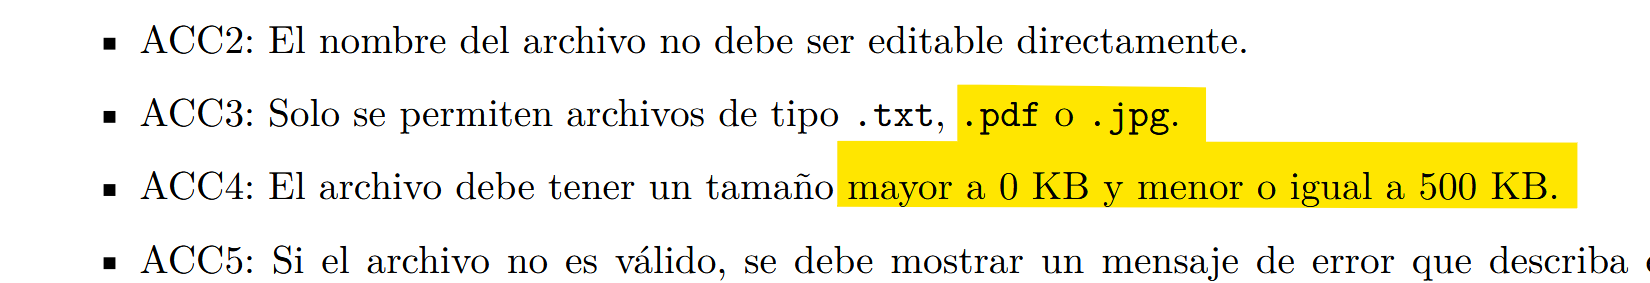
\includegraphics{images/ejercicio6.png}
  \caption{Ejercicio 6 - Criterios de aceptación}
  \label{fig:ejercicio6}
  Creo que hay un problema con el enunciado, ya que no es posible enviar adjuntos que no son \texttt{.txt} vacios.
  Por este motivo, he ponido solo un caso de prueba positivo, y tres negativos.
\end{figure}



\lstinputlisting[caption={Practica6.py}]{listings/Practica6.py}

\newpage

\subsection{Ejercicio 7 - Usuario bloqueado tras intentos fallidos de login}

Creo que hay un problema aquí también. El .pdf nos no da credenciales de prueba. He registrado un usuario de prueba, que pero no es permanente. Además, si el usuario se bloquea, no es posible desbloquearlo. 
Mi prueba ha funcionado, la primera vez que la he ejecutada, pero si vuelvo a ejecutarla falla.

\lstinputlisting[caption={Practica7.py}]{listings/Practica7.py}